\documentclass[1p]{elsarticle_modified}
%\bibliographystyle{elsarticle-num}

%\usepackage[colorlinks]{hyperref}
%\usepackage{abbrmath_seonhwa} %\Abb, \Ascr, \Acal ,\Abf, \Afrak
\usepackage{amsfonts}
\usepackage{amssymb}
\usepackage{amsmath}
\usepackage{amsthm}
\usepackage{scalefnt}
\usepackage{amsbsy}
\usepackage{kotex}
\usepackage{caption}
\usepackage{subfig}
\usepackage{color}
\usepackage{graphicx}
\usepackage{xcolor} %% white, black, red, green, blue, cyan, magenta, yellow
\usepackage{float}
\usepackage{setspace}
\usepackage{hyperref}

\usepackage{tikz}
\usetikzlibrary{arrows}

\usepackage{multirow}
\usepackage{array} % fixed length table
\usepackage{hhline}

%%%%%%%%%%%%%%%%%%%%%
\makeatletter
\renewcommand*\env@matrix[1][\arraystretch]{%
	\edef\arraystretch{#1}%
	\hskip -\arraycolsep
	\let\@ifnextchar\new@ifnextchar
	\array{*\c@MaxMatrixCols c}}
\makeatother %https://tex.stackexchange.com/questions/14071/how-can-i-increase-the-line-spacing-in-a-matrix
%%%%%%%%%%%%%%%

\usepackage[normalem]{ulem}

\newcommand{\msout}[1]{\ifmmode\text{\sout{\ensuremath{#1}}}\else\sout{#1}\fi}
%SOURCE: \msout is \stkout macro in https://tex.stackexchange.com/questions/20609/strikeout-in-math-mode

\newcommand{\cancel}[1]{
	\ifmmode
	{\color{red}\msout{#1}}
	\else
	{\color{red}\sout{#1}}
	\fi
}

\newcommand{\add}[1]{
	{\color{blue}\uwave{#1}}
}

\newcommand{\replace}[2]{
	\ifmmode
	{\color{red}\msout{#1}}{\color{blue}\uwave{#2}}
	\else
	{\color{red}\sout{#1}}{\color{blue}\uwave{#2}}
	\fi
}

\newcommand{\Sol}{\mathcal{S}} %segment
\newcommand{\D}{D} %diagram
\newcommand{\A}{\mathcal{A}} %arc


%%%%%%%%%%%%%%%%%%%%%%%%%%%%%5 test

\def\sl{\operatorname{\textup{SL}}(2,\Cbb)}
\def\psl{\operatorname{\textup{PSL}}(2,\Cbb)}
\def\quan{\mkern 1mu \triangleright \mkern 1mu}

\theoremstyle{definition}
\newtheorem{thm}{Theorem}[section]
\newtheorem{prop}[thm]{Proposition}
\newtheorem{lem}[thm]{Lemma}
\newtheorem{ques}[thm]{Question}
\newtheorem{cor}[thm]{Corollary}
\newtheorem{defn}[thm]{Definition}
\newtheorem{exam}[thm]{Example}
\newtheorem{rmk}[thm]{Remark}
\newtheorem{alg}[thm]{Algorithm}

\newcommand{\I}{\sqrt{-1}}
\begin{document}

%\begin{frontmatter}
%
%\title{Boundary parabolic representations of knots up to 8 crossings}
%
%%% Group authors per affiliation:
%\author{Yunhi Cho} 
%\address{Department of Mathematics, University of Seoul, Seoul, Korea}
%\ead{yhcho@uos.ac.kr}
%
%
%\author{Seonhwa Kim} %\fnref{s_kim}}
%\address{Center for Geometry and Physics, Institute for Basic Science, Pohang, 37673, Korea}
%\ead{ryeona17@ibs.re.kr}
%
%\author{Hyuk Kim}
%\address{Department of Mathematical Sciences, Seoul National University, Seoul 08826, Korea}
%\ead{hyukkim@snu.ac.kr}
%
%\author{Seokbeom Yoon}
%\address{Department of Mathematical Sciences, Seoul National University, Seoul, 08826,  Korea}
%\ead{sbyoon15@snu.ac.kr}
%
%\begin{abstract}
%We find all boundary parabolic representation of knots up to 8 crossings.
%
%\end{abstract}
%\begin{keyword}
%    \MSC[2010] 57M25 
%\end{keyword}
%
%\end{frontmatter}

%\linenumbers
%\tableofcontents
%
\newcommand\colored[1]{\textcolor{white}{\rule[-0.35ex]{0.8em}{1.4ex}}\kern-0.8em\color{red} #1}%
%\newcommand\colored[1]{\textcolor{white}{ #1}\kern-2.17ex	\textcolor{white}{ #1}\kern-1.81ex	\textcolor{white}{ #1}\kern-2.15ex\color{red}#1	}

{\Large $\underline{12n_{0765}~(K12n_{0765})}$}

\setlength{\tabcolsep}{10pt}
\renewcommand{\arraystretch}{1.6}
\vspace{1cm}\begin{tabular}{m{100pt}>{\centering\arraybackslash}m{274pt}}
\multirow{5}{120pt}{
	\centering
	\includegraphics[width=112pt]{../../../GIT/diagram.site/Diagrams/png/2854_12n_0765.png}\\
\ \ \ A knot diagram\footnotemark}&
\allowdisplaybreaks
\textbf{Linearized knot diagam} \\
\cline{2-2}
 &
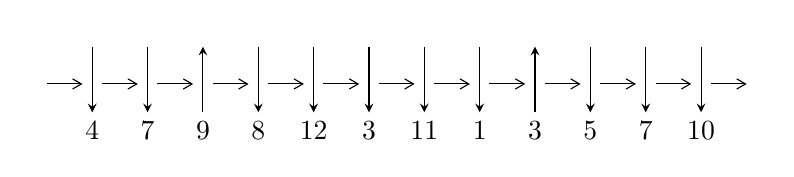
\begin{tikzpicture}[x=20pt, y=17pt]
	% nodes
	\node (C0) at (0, 0) {};
	\node (C1) at (1, 0) {};
	\node (C1U) at (1, +1) {};
	\node (C1D) at (1, -1) {4};

	\node (C2) at (2, 0) {};
	\node (C2U) at (2, +1) {};
	\node (C2D) at (2, -1) {7};

	\node (C3) at (3, 0) {};
	\node (C3U) at (3, +1) {};
	\node (C3D) at (3, -1) {9};

	\node (C4) at (4, 0) {};
	\node (C4U) at (4, +1) {};
	\node (C4D) at (4, -1) {8};

	\node (C5) at (5, 0) {};
	\node (C5U) at (5, +1) {};
	\node (C5D) at (5, -1) {12};

	\node (C6) at (6, 0) {};
	\node (C6U) at (6, +1) {};
	\node (C6D) at (6, -1) {3};

	\node (C7) at (7, 0) {};
	\node (C7U) at (7, +1) {};
	\node (C7D) at (7, -1) {11};

	\node (C8) at (8, 0) {};
	\node (C8U) at (8, +1) {};
	\node (C8D) at (8, -1) {1};

	\node (C9) at (9, 0) {};
	\node (C9U) at (9, +1) {};
	\node (C9D) at (9, -1) {3};

	\node (C10) at (10, 0) {};
	\node (C10U) at (10, +1) {};
	\node (C10D) at (10, -1) {5};

	\node (C11) at (11, 0) {};
	\node (C11U) at (11, +1) {};
	\node (C11D) at (11, -1) {7};

	\node (C12) at (12, 0) {};
	\node (C12U) at (12, +1) {};
	\node (C12D) at (12, -1) {10};
	\node (C13) at (13, 0) {};

	% arrows
	\draw[->,>={angle 60}]
	(C0) edge (C1) (C1) edge (C2) (C2) edge (C3) (C3) edge (C4) (C4) edge (C5) (C5) edge (C6) (C6) edge (C7) (C7) edge (C8) (C8) edge (C9) (C9) edge (C10) (C10) edge (C11) (C11) edge (C12) (C12) edge (C13) ;	\draw[->,>=stealth]
	(C1U) edge (C1D) (C2U) edge (C2D) (C3D) edge (C3U) (C4U) edge (C4D) (C5U) edge (C5D) (C6U) edge (C6D) (C7U) edge (C7D) (C8U) edge (C8D) (C9D) edge (C9U) (C10U) edge (C10D) (C11U) edge (C11D) (C12U) edge (C12D) ;
	\end{tikzpicture} \\
\hhline{~~} \\& 
\textbf{Solving Sequence} \\ \cline{2-2} 
 &
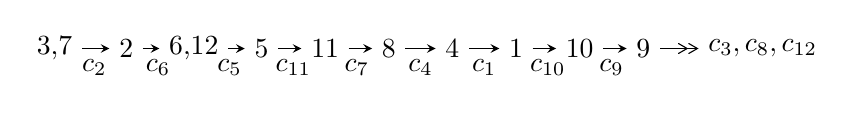
\begin{tikzpicture}[x=23pt, y=7pt]
	% node
	\node (A0) at (-1/8, 0) {3,7};
	\node (A1) at (1, 0) {2};
	\node (A2) at (33/16, 0) {6,12};
	\node (A3) at (25/8, 0) {5};
	\node (A4) at (33/8, 0) {11};
	\node (A5) at (41/8, 0) {8};
	\node (A6) at (49/8, 0) {4};
	\node (A7) at (57/8, 0) {1};
	\node (A8) at (65/8, 0) {10};
	\node (A9) at (73/8, 0) {9};
	\node (C1) at (1/2, -1) {$c_{2}$};
	\node (C2) at (3/2, -1) {$c_{6}$};
	\node (C3) at (21/8, -1) {$c_{5}$};
	\node (C4) at (29/8, -1) {$c_{11}$};
	\node (C5) at (37/8, -1) {$c_{7}$};
	\node (C6) at (45/8, -1) {$c_{4}$};
	\node (C7) at (53/8, -1) {$c_{1}$};
	\node (C8) at (61/8, -1) {$c_{10}$};
	\node (C9) at (69/8, -1) {$c_{9}$};
	\node (A10) at (11, 0) {$c_{3},c_{8},c_{12}$};

	% edge
	\draw[->,>=stealth]	
	(A0) edge (A1) (A1) edge (A2) (A2) edge (A3) (A3) edge (A4) (A4) edge (A5) (A5) edge (A6) (A6) edge (A7) (A7) edge (A8) (A8) edge (A9) ;
	\draw[->>,>={angle 60}]	
	(A9) edge (A10);
\end{tikzpicture} \\ 

\end{tabular} \\

\footnotetext{
The image of knot diagram is generated by the software ``\textbf{Draw programme}" developed by Andrew Bartholomew(\url{http://www.layer8.co.uk/maths/draw/index.htm\#Running-draw}), where we modified some parts for our purpose(\url{https://github.com/CATsTAILs/LinksPainter}).
}\phantom \\ \newline 
\centering \textbf{Ideals for irreducible components\footnotemark of $X_{\text{par}}$} 
 
\begin{align*}
I^u_{1}&=\langle 
-1.60013\times10^{687} u^{108}+5.32223\times10^{687} u^{107}+\cdots+1.17704\times10^{692} b-5.63654\times10^{692},\\
\phantom{I^u_{1}}&\phantom{= \langle  }-8.49812\times10^{693} u^{108}+3.39185\times10^{694} u^{107}+\cdots+4.81217\times10^{697} a-3.97557\times10^{699},\\
\phantom{I^u_{1}}&\phantom{= \langle  }u^{109}-4 u^{108}+\cdots+727773 u-58405\rangle \\
I^u_{2}&=\langle 
3.87954\times10^{45} u^{40}-3.63289\times10^{45} u^{39}+\cdots+7.89408\times10^{44} b+9.18467\times10^{44},\\
\phantom{I^u_{2}}&\phantom{= \langle  }7.60703\times10^{44} u^{40}+4.49925\times10^{45} u^{39}+\cdots+7.89408\times10^{44} a-1.27861\times10^{46},\;u^{41}- u^{40}+\cdots+3 u-1\rangle \\
\\
\end{align*}
\raggedright * 2 irreducible components of $\dim_{\mathbb{C}}=0$, with total 150 representations.\\
\footnotetext{All coefficients of polynomials are rational numbers. But the coefficients are sometimes approximated in decimal forms when there is not enough margin.}
\newpage
\renewcommand{\arraystretch}{1}
\centering \section*{I. $I^u_{1}= \langle -1.60\times10^{687} u^{108}+5.32\times10^{687} u^{107}+\cdots+1.18\times10^{692} b-5.64\times10^{692},\;-8.50\times10^{693} u^{108}+3.39\times10^{694} u^{107}+\cdots+4.81\times10^{697} a-3.98\times10^{699},\;u^{109}-4 u^{108}+\cdots+727773 u-58405 \rangle$}
\flushleft \textbf{(i) Arc colorings}\\
\begin{tabular}{m{7pt} m{180pt} m{7pt} m{180pt} }
\flushright $a_{3}=$&$\begin{pmatrix}1\\0\end{pmatrix}$ \\
\flushright $a_{7}=$&$\begin{pmatrix}0\\u\end{pmatrix}$ \\
\flushright $a_{2}=$&$\begin{pmatrix}1\\- u^2\end{pmatrix}$ \\
\flushright $a_{6}=$&$\begin{pmatrix}u\\u\end{pmatrix}$ \\
\flushright $a_{12}=$&$\begin{pmatrix}0.000176596 u^{108}-0.000704848 u^{107}+\cdots-536.559 u+82.6149\\0.0000135945 u^{108}-0.0000452169 u^{107}+\cdots-24.5059 u+4.78872\end{pmatrix}$ \\
\flushright $a_{5}=$&$\begin{pmatrix}0.00109313 u^{108}-0.00409347 u^{107}+\cdots-2133.44 u+244.622\\0.000218812 u^{108}-0.000804043 u^{107}+\cdots-378.582 u+40.3302\end{pmatrix}$ \\
\flushright $a_{11}=$&$\begin{pmatrix}0.000176596 u^{108}-0.000704848 u^{107}+\cdots-536.559 u+82.6149\\0.0000211796 u^{108}-0.0000731613 u^{107}+\cdots-33.7006 u+4.69889\end{pmatrix}$ \\
\flushright $a_{8}=$&$\begin{pmatrix}-0.00135482 u^{108}+0.00506301 u^{107}+\cdots+2607.30 u-295.218\\-0.000168745 u^{108}+0.000622795 u^{107}+\cdots+293.699 u-29.7884\end{pmatrix}$ \\
\flushright $a_{4}=$&$\begin{pmatrix}0.000223168 u^{108}-0.000792062 u^{107}+\cdots-244.124 u+12.4619\\-0.000137835 u^{108}+0.000517495 u^{107}+\cdots+286.997 u-36.5128\end{pmatrix}$ \\
\flushright $a_{1}=$&$\begin{pmatrix}-0.00112968 u^{108}+0.00417253 u^{107}+\cdots+1958.79 u-197.708\\-0.000171027 u^{108}+0.000635449 u^{107}+\cdots+296.271 u-28.3214\end{pmatrix}$ \\
\flushright $a_{10}=$&$\begin{pmatrix}-0.000757974 u^{108}+0.00281956 u^{107}+\cdots+1391.84 u-148.178\\-0.000213592 u^{108}+0.000799611 u^{107}+\cdots+408.288 u-45.4695\end{pmatrix}$ \\
\flushright $a_{9}=$&$\begin{pmatrix}-0.000544383 u^{108}+0.00201995 u^{107}+\cdots+983.548 u-102.709\\-0.000213592 u^{108}+0.000799611 u^{107}+\cdots+408.288 u-45.4695\end{pmatrix}$\\&\end{tabular}
\flushleft \textbf{(ii) Obstruction class $= -1$}\\~\\
\flushleft \textbf{(iii) Cusp Shapes $= 0.0000966670 u^{108}-0.000299148 u^{107}+\cdots+79.9719 u-45.9238$}\\~\\
\newpage\renewcommand{\arraystretch}{1}
\flushleft \textbf{(iv) u-Polynomials at the component}\newline \\
\begin{tabular}{m{50pt}|m{274pt}}
Crossings & \hspace{64pt}u-Polynomials at each crossing \\
\hline $$\begin{aligned}c_{1}\end{aligned}$$&$\begin{aligned}
&u^{109}-5 u^{108}+\cdots+2849220 u-293753
\end{aligned}$\\
\hline $$\begin{aligned}c_{2},c_{6}\end{aligned}$$&$\begin{aligned}
&u^{109}+4 u^{108}+\cdots+727773 u+58405
\end{aligned}$\\
\hline $$\begin{aligned}c_{3},c_{9}\end{aligned}$$&$\begin{aligned}
&u^{109}+u^{108}+\cdots+18828 u+2079
\end{aligned}$\\
\hline $$\begin{aligned}c_{4}\end{aligned}$$&$\begin{aligned}
&u^{109}+4 u^{108}+\cdots-24796 u+1679
\end{aligned}$\\
\hline $$\begin{aligned}c_{5}\end{aligned}$$&$\begin{aligned}
&u^{109}+u^{108}+\cdots-1214779937 u+75810647
\end{aligned}$\\
\hline $$\begin{aligned}c_{7},c_{11}\end{aligned}$$&$\begin{aligned}
&u^{109}+3 u^{108}+\cdots+4565 u+4481
\end{aligned}$\\
\hline $$\begin{aligned}c_{8}\end{aligned}$$&$\begin{aligned}
&u^{109}+2 u^{108}+\cdots-13 u+1
\end{aligned}$\\
\hline $$\begin{aligned}c_{10}\end{aligned}$$&$\begin{aligned}
&u^{109}+u^{108}+\cdots+4838 u+2189
\end{aligned}$\\
\hline $$\begin{aligned}c_{12}\end{aligned}$$&$\begin{aligned}
&u^{109}-8 u^{108}+\cdots-2468184 u+292253
\end{aligned}$\\
\hline
\end{tabular}\\~\\
\newpage\renewcommand{\arraystretch}{1}
\flushleft \textbf{(v) Riley Polynomials at the component}\newline \\
\begin{tabular}{m{50pt}|m{274pt}}
Crossings & \hspace{64pt}Riley Polynomials at each crossing \\
\hline $$\begin{aligned}c_{1}\end{aligned}$$&$\begin{aligned}
&y^{109}-33 y^{108}+\cdots+7391217447958 y-86290825009
\end{aligned}$\\
\hline $$\begin{aligned}c_{2},c_{6}\end{aligned}$$&$\begin{aligned}
&y^{109}-78 y^{108}+\cdots+176189049349 y-3411144025
\end{aligned}$\\
\hline $$\begin{aligned}c_{3},c_{9}\end{aligned}$$&$\begin{aligned}
&y^{109}+93 y^{108}+\cdots-38599578 y-4322241
\end{aligned}$\\
\hline $$\begin{aligned}c_{4}\end{aligned}$$&$\begin{aligned}
&y^{109}+22 y^{108}+\cdots+390164552 y-2819041
\end{aligned}$\\
\hline $$\begin{aligned}c_{5}\end{aligned}$$&$\begin{aligned}
&y^{109}-21 y^{108}+\cdots+602106898292238931 y-5747254198558609
\end{aligned}$\\
\hline $$\begin{aligned}c_{7},c_{11}\end{aligned}$$&$\begin{aligned}
&y^{109}+61 y^{108}+\cdots-397560707 y-20079361
\end{aligned}$\\
\hline $$\begin{aligned}c_{8}\end{aligned}$$&$\begin{aligned}
&y^{109}+14 y^{108}+\cdots+9 y-1
\end{aligned}$\\
\hline $$\begin{aligned}c_{10}\end{aligned}$$&$\begin{aligned}
&y^{109}+45 y^{108}+\cdots-112723288 y-4791721
\end{aligned}$\\
\hline $$\begin{aligned}c_{12}\end{aligned}$$&$\begin{aligned}
&y^{109}-34 y^{108}+\cdots-684202546700 y-85411816009
\end{aligned}$\\
\hline
\end{tabular}\\~\\
\newpage\flushleft \textbf{(vi) Complex Volumes and Cusp Shapes}
$$\begin{array}{c|c|c}  
\text{Solutions to }I^u_{1}& \I (\text{vol} + \sqrt{-1}CS) & \text{Cusp shape}\\
 \hline 
\begin{aligned}
u &= -0.937174 + 0.281919 I \\
a &= -0.230672 + 0.213488 I \\
b &= -1.49885 - 0.38451 I\end{aligned}
 & -4.58867 - 4.06930 I & \phantom{-0.000000 } 0 \\ \hline\begin{aligned}
u &= -0.937174 - 0.281919 I \\
a &= -0.230672 - 0.213488 I \\
b &= -1.49885 + 0.38451 I\end{aligned}
 & -4.58867 + 4.06930 I & \phantom{-0.000000 } 0 \\ \hline\begin{aligned}
u &= \phantom{-}1.080690 + 0.035625 I \\
a &= -0.263367 - 1.153200 I \\
b &= -1.52630 + 0.80230 I\end{aligned}
 & \phantom{-}1.60982 - 2.70191 I & \phantom{-0.000000 } 0 \\ \hline\begin{aligned}
u &= \phantom{-}1.080690 - 0.035625 I \\
a &= -0.263367 + 1.153200 I \\
b &= -1.52630 - 0.80230 I\end{aligned}
 & \phantom{-}1.60982 + 2.70191 I & \phantom{-0.000000 } 0 \\ \hline\begin{aligned}
u &= \phantom{-}0.409206 + 0.822293 I \\
a &= \phantom{-}1.220430 + 0.422812 I \\
b &= \phantom{-}0.725883 - 0.641836 I\end{aligned}
 & \phantom{-}2.78846 - 3.45010 I & \phantom{-0.000000 } 0 \\ \hline\begin{aligned}
u &= \phantom{-}0.409206 - 0.822293 I \\
a &= \phantom{-}1.220430 - 0.422812 I \\
b &= \phantom{-}0.725883 + 0.641836 I\end{aligned}
 & \phantom{-}2.78846 + 3.45010 I & \phantom{-0.000000 } 0 \\ \hline\begin{aligned}
u &= -0.253662 + 1.058760 I \\
a &= \phantom{-}0.751003 + 0.041761 I \\
b &= \phantom{-}1.181380 + 0.618099 I\end{aligned}
 & \phantom{-}2.83743 + 3.68107 I & \phantom{-0.000000 } 0 \\ \hline\begin{aligned}
u &= -0.253662 - 1.058760 I \\
a &= \phantom{-}0.751003 - 0.041761 I \\
b &= \phantom{-}1.181380 - 0.618099 I\end{aligned}
 & \phantom{-}2.83743 - 3.68107 I & \phantom{-0.000000 } 0 \\ \hline\begin{aligned}
u &= -1.134750 + 0.112447 I \\
a &= -1.061230 - 0.411871 I \\
b &= -1.71856 - 0.12374 I\end{aligned}
 & -3.71782 + 0.50102 I & \phantom{-0.000000 } 0 \\ \hline\begin{aligned}
u &= -1.134750 - 0.112447 I \\
a &= -1.061230 + 0.411871 I \\
b &= -1.71856 + 0.12374 I\end{aligned}
 & -3.71782 - 0.50102 I & \phantom{-0.000000 } 0\\
 \hline 
 \end{array}$$\newpage$$\begin{array}{c|c|c}  
\text{Solutions to }I^u_{1}& \I (\text{vol} + \sqrt{-1}CS) & \text{Cusp shape}\\
 \hline 
\begin{aligned}
u &= -0.165462 + 0.833409 I \\
a &= -0.255766 + 0.833211 I \\
b &= -0.640398 - 0.315196 I\end{aligned}
 & -4.30464 - 3.55844 I & \phantom{-0.000000 } 0 \\ \hline\begin{aligned}
u &= -0.165462 - 0.833409 I \\
a &= -0.255766 - 0.833211 I \\
b &= -0.640398 + 0.315196 I\end{aligned}
 & -4.30464 + 3.55844 I & \phantom{-0.000000 } 0 \\ \hline\begin{aligned}
u &= \phantom{-}0.015038 + 0.819293 I \\
a &= -0.017611 + 0.689819 I \\
b &= \phantom{-}0.794081 - 0.256196 I\end{aligned}
 & \phantom{-}2.65946 - 2.53857 I & \phantom{-0.000000 } 0 \\ \hline\begin{aligned}
u &= \phantom{-}0.015038 - 0.819293 I \\
a &= -0.017611 - 0.689819 I \\
b &= \phantom{-}0.794081 + 0.256196 I\end{aligned}
 & \phantom{-}2.65946 + 2.53857 I & \phantom{-0.000000 } 0 \\ \hline\begin{aligned}
u &= \phantom{-}1.218700 + 0.061079 I \\
a &= -0.327349 - 0.045298 I \\
b &= -0.971741 - 0.281094 I\end{aligned}
 & -2.01895 + 0.10579 I & \phantom{-0.000000 } 0 \\ \hline\begin{aligned}
u &= \phantom{-}1.218700 - 0.061079 I \\
a &= -0.327349 + 0.045298 I \\
b &= -0.971741 + 0.281094 I\end{aligned}
 & -2.01895 - 0.10579 I & \phantom{-0.000000 } 0 \\ \hline\begin{aligned}
u &= \phantom{-}1.192660 + 0.290351 I \\
a &= -0.282359 - 0.722232 I \\
b &= -1.47325 - 0.75659 I\end{aligned}
 & -0.360070 - 0.634714 I & \phantom{-0.000000 } 0 \\ \hline\begin{aligned}
u &= \phantom{-}1.192660 - 0.290351 I \\
a &= -0.282359 + 0.722232 I \\
b &= -1.47325 + 0.75659 I\end{aligned}
 & -0.360070 + 0.634714 I & \phantom{-0.000000 } 0 \\ \hline\begin{aligned}
u &= \phantom{-}1.175000 + 0.393607 I \\
a &= -1.397410 + 0.013308 I \\
b &= -1.93087 + 0.00761 I\end{aligned}
 & -7.33757 - 1.84736 I & \phantom{-0.000000 } 0 \\ \hline\begin{aligned}
u &= \phantom{-}1.175000 - 0.393607 I \\
a &= -1.397410 - 0.013308 I \\
b &= -1.93087 - 0.00761 I\end{aligned}
 & -7.33757 + 1.84736 I & \phantom{-0.000000 } 0\\
 \hline 
 \end{array}$$\newpage$$\begin{array}{c|c|c}  
\text{Solutions to }I^u_{1}& \I (\text{vol} + \sqrt{-1}CS) & \text{Cusp shape}\\
 \hline 
\begin{aligned}
u &= \phantom{-}1.189630 + 0.361967 I \\
a &= -0.424286 - 0.392824 I \\
b &= -1.384160 - 0.097087 I\end{aligned}
 & -1.73331 - 0.64522 I & \phantom{-0.000000 } 0 \\ \hline\begin{aligned}
u &= \phantom{-}1.189630 - 0.361967 I \\
a &= -0.424286 + 0.392824 I \\
b &= -1.384160 + 0.097087 I\end{aligned}
 & -1.73331 + 0.64522 I & \phantom{-0.000000 } 0 \\ \hline\begin{aligned}
u &= \phantom{-}0.156542 + 0.710487 I \\
a &= -1.84667 - 0.16232 I \\
b &= \phantom{-}0.0461817 - 0.1138670 I\end{aligned}
 & \phantom{-}6.82913 - 5.20735 I & \phantom{-}7.39068 + 8.40503 I \\ \hline\begin{aligned}
u &= \phantom{-}0.156542 - 0.710487 I \\
a &= -1.84667 + 0.16232 I \\
b &= \phantom{-}0.0461817 + 0.1138670 I\end{aligned}
 & \phantom{-}6.82913 + 5.20735 I & \phantom{-}7.39068 - 8.40503 I \\ \hline\begin{aligned}
u &= -0.524309 + 0.479493 I \\
a &= -1.04314 + 1.55348 I \\
b &= \phantom{-}0.389923 + 0.440071 I\end{aligned}
 & \phantom{-}4.99089 + 1.89299 I & -3.93271 - 5.59425 I \\ \hline\begin{aligned}
u &= -0.524309 - 0.479493 I \\
a &= -1.04314 - 1.55348 I \\
b &= \phantom{-}0.389923 - 0.440071 I\end{aligned}
 & \phantom{-}4.99089 - 1.89299 I & -3.93271 + 5.59425 I \\ \hline\begin{aligned}
u &= -0.674783 + 0.207559 I \\
a &= \phantom{-}1.02731 - 1.07769 I \\
b &= \phantom{-}0.43795 - 1.51100 I\end{aligned}
 & \phantom{-}4.55542 + 0.50960 I & -3.96864 - 4.23818 I \\ \hline\begin{aligned}
u &= -0.674783 - 0.207559 I \\
a &= \phantom{-}1.02731 + 1.07769 I \\
b &= \phantom{-}0.43795 + 1.51100 I\end{aligned}
 & \phantom{-}4.55542 - 0.50960 I & -3.96864 + 4.23818 I \\ \hline\begin{aligned}
u &= \phantom{-}0.406321 + 1.252440 I \\
a &= -0.405878 - 0.240420 I \\
b &= -0.391235 - 0.535451 I\end{aligned}
 & \phantom{-}0.41060 - 2.38012 I & \phantom{-0.000000 } 0 \\ \hline\begin{aligned}
u &= \phantom{-}0.406321 - 1.252440 I \\
a &= -0.405878 + 0.240420 I \\
b &= -0.391235 + 0.535451 I\end{aligned}
 & \phantom{-}0.41060 + 2.38012 I & \phantom{-0.000000 } 0\\
 \hline 
 \end{array}$$\newpage$$\begin{array}{c|c|c}  
\text{Solutions to }I^u_{1}& \I (\text{vol} + \sqrt{-1}CS) & \text{Cusp shape}\\
 \hline 
\begin{aligned}
u &= -1.337270 + 0.096420 I \\
a &= \phantom{-}0.780139 + 0.431312 I \\
b &= \phantom{-}1.57724 - 0.09865 I\end{aligned}
 & -1.87689 + 5.25392 I & \phantom{-0.000000 } 0 \\ \hline\begin{aligned}
u &= -1.337270 - 0.096420 I \\
a &= \phantom{-}0.780139 - 0.431312 I \\
b &= \phantom{-}1.57724 + 0.09865 I\end{aligned}
 & -1.87689 - 5.25392 I & \phantom{-0.000000 } 0 \\ \hline\begin{aligned}
u &= \phantom{-}1.189590 + 0.623116 I \\
a &= \phantom{-}0.718724 + 0.455567 I \\
b &= \phantom{-}1.408480 - 0.013907 I\end{aligned}
 & -1.82505 - 3.69562 I & \phantom{-0.000000 } 0 \\ \hline\begin{aligned}
u &= \phantom{-}1.189590 - 0.623116 I \\
a &= \phantom{-}0.718724 - 0.455567 I \\
b &= \phantom{-}1.408480 + 0.013907 I\end{aligned}
 & -1.82505 + 3.69562 I & \phantom{-0.000000 } 0 \\ \hline\begin{aligned}
u &= \phantom{-}1.341710 + 0.078743 I \\
a &= \phantom{-}0.156215 + 1.349690 I \\
b &= \phantom{-}0.344551 + 0.035975 I\end{aligned}
 & -0.22447 + 4.16339 I & \phantom{-0.000000 } 0 \\ \hline\begin{aligned}
u &= \phantom{-}1.341710 - 0.078743 I \\
a &= \phantom{-}0.156215 - 1.349690 I \\
b &= \phantom{-}0.344551 - 0.035975 I\end{aligned}
 & -0.22447 - 4.16339 I & \phantom{-0.000000 } 0 \\ \hline\begin{aligned}
u &= -1.278060 + 0.462387 I \\
a &= -0.762034 + 0.734670 I \\
b &= -1.66970 + 0.93674 I\end{aligned}
 & -0.48833 + 7.00109 I & \phantom{-0.000000 } 0 \\ \hline\begin{aligned}
u &= -1.278060 - 0.462387 I \\
a &= -0.762034 - 0.734670 I \\
b &= -1.66970 - 0.93674 I\end{aligned}
 & -0.48833 - 7.00109 I & \phantom{-0.000000 } 0 \\ \hline\begin{aligned}
u &= \phantom{-}0.352130 + 0.512930 I \\
a &= \phantom{-}0.724990 - 0.800184 I \\
b &= -0.109651 - 0.352445 I\end{aligned}
 & -1.54116 - 1.08486 I & -13.13256 + 3.91208 I \\ \hline\begin{aligned}
u &= \phantom{-}0.352130 - 0.512930 I \\
a &= \phantom{-}0.724990 + 0.800184 I \\
b &= -0.109651 + 0.352445 I\end{aligned}
 & -1.54116 + 1.08486 I & -13.13256 - 3.91208 I\\
 \hline 
 \end{array}$$\newpage$$\begin{array}{c|c|c}  
\text{Solutions to }I^u_{1}& \I (\text{vol} + \sqrt{-1}CS) & \text{Cusp shape}\\
 \hline 
\begin{aligned}
u &= -1.357060 + 0.289480 I \\
a &= -0.542508 + 0.846957 I \\
b &= -1.52610 + 0.94254 I\end{aligned}
 & -0.66014 + 7.54621 I & \phantom{-0.000000 } 0 \\ \hline\begin{aligned}
u &= -1.357060 - 0.289480 I \\
a &= -0.542508 - 0.846957 I \\
b &= -1.52610 - 0.94254 I\end{aligned}
 & -0.66014 - 7.54621 I & \phantom{-0.000000 } 0 \\ \hline\begin{aligned}
u &= -1.376720 + 0.267957 I \\
a &= -0.845102 + 0.485644 I \\
b &= -1.77518 + 0.33114 I\end{aligned}
 & -6.44692 + 3.80582 I & \phantom{-0.000000 } 0 \\ \hline\begin{aligned}
u &= -1.376720 - 0.267957 I \\
a &= -0.845102 - 0.485644 I \\
b &= -1.77518 - 0.33114 I\end{aligned}
 & -6.44692 - 3.80582 I & \phantom{-0.000000 } 0 \\ \hline\begin{aligned}
u &= -0.559578 + 0.198192 I \\
a &= -1.22023 + 1.28236 I \\
b &= -0.35442 + 2.58430 I\end{aligned}
 & \phantom{-}2.52276 + 7.95086 I & -9.5091 - 11.5695 I \\ \hline\begin{aligned}
u &= -0.559578 - 0.198192 I \\
a &= -1.22023 - 1.28236 I \\
b &= -0.35442 - 2.58430 I\end{aligned}
 & \phantom{-}2.52276 - 7.95086 I & -9.5091 + 11.5695 I \\ \hline\begin{aligned}
u &= -1.398260 + 0.151811 I \\
a &= \phantom{-}0.496418 - 0.584354 I \\
b &= \phantom{-}1.67339 + 0.17878 I\end{aligned}
 & -7.33133 - 3.59033 I & \phantom{-0.000000 } 0 \\ \hline\begin{aligned}
u &= -1.398260 - 0.151811 I \\
a &= \phantom{-}0.496418 + 0.584354 I \\
b &= \phantom{-}1.67339 - 0.17878 I\end{aligned}
 & -7.33133 + 3.59033 I & \phantom{-0.000000 } 0 \\ \hline\begin{aligned}
u &= \phantom{-}0.452974 + 1.335320 I \\
a &= \phantom{-}0.644020 + 0.629180 I \\
b &= \phantom{-}0.369458 - 0.468319 I\end{aligned}
 & -2.07029 + 1.11942 I & \phantom{-0.000000 } 0 \\ \hline\begin{aligned}
u &= \phantom{-}0.452974 - 1.335320 I \\
a &= \phantom{-}0.644020 - 0.629180 I \\
b &= \phantom{-}0.369458 + 0.468319 I\end{aligned}
 & -2.07029 - 1.11942 I & \phantom{-0.000000 } 0\\
 \hline 
 \end{array}$$\newpage$$\begin{array}{c|c|c}  
\text{Solutions to }I^u_{1}& \I (\text{vol} + \sqrt{-1}CS) & \text{Cusp shape}\\
 \hline 
\begin{aligned}
u &= -0.187385 + 0.556680 I \\
a &= \phantom{-}1.83950 - 1.14234 I \\
b &= \phantom{-}0.098192 - 0.307884 I\end{aligned}
 & \phantom{-}2.65011 - 2.82680 I & -3.87963 + 2.53461 I \\ \hline\begin{aligned}
u &= -0.187385 - 0.556680 I \\
a &= \phantom{-}1.83950 + 1.14234 I \\
b &= \phantom{-}0.098192 + 0.307884 I\end{aligned}
 & \phantom{-}2.65011 + 2.82680 I & -3.87963 - 2.53461 I \\ \hline\begin{aligned}
u &= \phantom{-}1.42705 + 0.10899 I \\
a &= -0.692128 - 0.933953 I \\
b &= -1.32045 - 0.69634 I\end{aligned}
 & -4.12477 - 6.75342 I & \phantom{-0.000000 } 0 \\ \hline\begin{aligned}
u &= \phantom{-}1.42705 - 0.10899 I \\
a &= -0.692128 + 0.933953 I \\
b &= -1.32045 + 0.69634 I\end{aligned}
 & -4.12477 + 6.75342 I & \phantom{-0.000000 } 0 \\ \hline\begin{aligned}
u &= \phantom{-}0.21991 + 1.44095 I \\
a &= \phantom{-}0.661564 + 0.133231 I \\
b &= \phantom{-}0.646671 + 0.016763 I\end{aligned}
 & \phantom{-}5.71970 - 3.02646 I & \phantom{-0.000000 } 0 \\ \hline\begin{aligned}
u &= \phantom{-}0.21991 - 1.44095 I \\
a &= \phantom{-}0.661564 - 0.133231 I \\
b &= \phantom{-}0.646671 - 0.016763 I\end{aligned}
 & \phantom{-}5.71970 + 3.02646 I & \phantom{-0.000000 } 0 \\ \hline\begin{aligned}
u &= \phantom{-}0.514423 + 0.169978 I \\
a &= -0.93648 - 1.06633 I \\
b &= \phantom{-}1.04253 - 1.61461 I\end{aligned}
 & \phantom{-}3.58991 - 2.77762 I & -8.20669 + 3.30808 I \\ \hline\begin{aligned}
u &= \phantom{-}0.514423 - 0.169978 I \\
a &= -0.93648 + 1.06633 I \\
b &= \phantom{-}1.04253 + 1.61461 I\end{aligned}
 & \phantom{-}3.58991 + 2.77762 I & -8.20669 - 3.30808 I \\ \hline\begin{aligned}
u &= \phantom{-}0.524647 + 0.037159 I \\
a &= \phantom{-}0.75002 + 1.84238 I \\
b &= -0.77378 + 2.20253 I\end{aligned}
 & \phantom{-}2.68546 + 4.66613 I & -10.91912 - 1.69700 I \\ \hline\begin{aligned}
u &= \phantom{-}0.524647 - 0.037159 I \\
a &= \phantom{-}0.75002 - 1.84238 I \\
b &= -0.77378 - 2.20253 I\end{aligned}
 & \phantom{-}2.68546 - 4.66613 I & -10.91912 + 1.69700 I\\
 \hline 
 \end{array}$$\newpage$$\begin{array}{c|c|c}  
\text{Solutions to }I^u_{1}& \I (\text{vol} + \sqrt{-1}CS) & \text{Cusp shape}\\
 \hline 
\begin{aligned}
u &= -1.41447 + 0.57889 I \\
a &= -0.715649 + 0.423665 I \\
b &= -1.69115 + 0.21932 I\end{aligned}
 & -6.68545 + 4.08833 I & \phantom{-0.000000 } 0 \\ \hline\begin{aligned}
u &= -1.41447 - 0.57889 I \\
a &= -0.715649 - 0.423665 I \\
b &= -1.69115 - 0.21932 I\end{aligned}
 & -6.68545 - 4.08833 I & \phantom{-0.000000 } 0 \\ \hline\begin{aligned}
u &= -0.14362 + 1.52726 I \\
a &= -0.540609 + 0.275968 I \\
b &= -0.355021 - 0.067337 I\end{aligned}
 & \phantom{-}5.37904 - 4.69106 I & \phantom{-0.000000 } 0 \\ \hline\begin{aligned}
u &= -0.14362 - 1.52726 I \\
a &= -0.540609 - 0.275968 I \\
b &= -0.355021 + 0.067337 I\end{aligned}
 & \phantom{-}5.37904 + 4.69106 I & \phantom{-0.000000 } 0 \\ \hline\begin{aligned}
u &= \phantom{-}1.54337 + 0.10690 I \\
a &= \phantom{-}0.257980 - 0.420750 I \\
b &= \phantom{-}0.779436 - 0.674871 I\end{aligned}
 & -3.07896 + 0.61761 I & \phantom{-0.000000 } 0 \\ \hline\begin{aligned}
u &= \phantom{-}1.54337 - 0.10690 I \\
a &= \phantom{-}0.257980 + 0.420750 I \\
b &= \phantom{-}0.779436 + 0.674871 I\end{aligned}
 & -3.07896 - 0.61761 I & \phantom{-0.000000 } 0 \\ \hline\begin{aligned}
u &= \phantom{-}1.54678 + 0.17407 I \\
a &= -0.384794 - 0.630950 I \\
b &= -1.210880 - 0.658366 I\end{aligned}
 & -0.26332 - 3.09618 I & \phantom{-0.000000 } 0 \\ \hline\begin{aligned}
u &= \phantom{-}1.54678 - 0.17407 I \\
a &= -0.384794 + 0.630950 I \\
b &= -1.210880 + 0.658366 I\end{aligned}
 & -0.26332 + 3.09618 I & \phantom{-0.000000 } 0 \\ \hline\begin{aligned}
u &= -0.158026 + 0.411664 I \\
a &= \phantom{-}2.88876 - 1.73873 I \\
b &= \phantom{-}0.531342 - 0.090450 I\end{aligned}
 & \phantom{-}3.79386 - 4.83112 I & -10.98344 - 3.75502 I \\ \hline\begin{aligned}
u &= -0.158026 - 0.411664 I \\
a &= \phantom{-}2.88876 + 1.73873 I \\
b &= \phantom{-}0.531342 + 0.090450 I\end{aligned}
 & \phantom{-}3.79386 + 4.83112 I & -10.98344 + 3.75502 I\\
 \hline 
 \end{array}$$\newpage$$\begin{array}{c|c|c}  
\text{Solutions to }I^u_{1}& \I (\text{vol} + \sqrt{-1}CS) & \text{Cusp shape}\\
 \hline 
\begin{aligned}
u &= -1.55527 + 0.16816 I \\
a &= -0.039347 - 0.948769 I \\
b &= -0.619397 + 1.178490 I\end{aligned}
 & -1.01007 - 5.69221 I & \phantom{-0.000000 } 0 \\ \hline\begin{aligned}
u &= -1.55527 - 0.16816 I \\
a &= -0.039347 + 0.948769 I \\
b &= -0.619397 - 1.178490 I\end{aligned}
 & -1.01007 + 5.69221 I & \phantom{-0.000000 } 0 \\ \hline\begin{aligned}
u &= \phantom{-}1.50449 + 0.46131 I \\
a &= \phantom{-}0.837670 + 0.417346 I \\
b &= \phantom{-}1.381910 + 0.237508 I\end{aligned}
 & -4.44221 - 4.06401 I & \phantom{-0.000000 } 0 \\ \hline\begin{aligned}
u &= \phantom{-}1.50449 - 0.46131 I \\
a &= \phantom{-}0.837670 - 0.417346 I \\
b &= \phantom{-}1.381910 - 0.237508 I\end{aligned}
 & -4.44221 + 4.06401 I & \phantom{-0.000000 } 0 \\ \hline\begin{aligned}
u &= -1.56004 + 0.23230 I \\
a &= -0.297932 + 0.558155 I \\
b &= -1.75199 + 0.30606 I\end{aligned}
 & -2.53673 + 1.36112 I & \phantom{-0.000000 } 0 \\ \hline\begin{aligned}
u &= -1.56004 - 0.23230 I \\
a &= -0.297932 - 0.558155 I \\
b &= -1.75199 - 0.30606 I\end{aligned}
 & -2.53673 - 1.36112 I & \phantom{-0.000000 } 0 \\ \hline\begin{aligned}
u &= \phantom{-}0.240074 + 0.345112 I \\
a &= \phantom{-}1.052540 - 0.125492 I \\
b &= \phantom{-}0.070492 - 0.493744 I\end{aligned}
 & -0.626116 - 1.232790 I & -6.62259 + 5.91727 I \\ \hline\begin{aligned}
u &= \phantom{-}0.240074 - 0.345112 I \\
a &= \phantom{-}1.052540 + 0.125492 I \\
b &= \phantom{-}0.070492 + 0.493744 I\end{aligned}
 & -0.626116 + 1.232790 I & -6.62259 - 5.91727 I \\ \hline\begin{aligned}
u &= -1.34419 + 0.86246 I \\
a &= \phantom{-}0.655259 - 0.415772 I \\
b &= \phantom{-}1.55924 - 0.19368 I\end{aligned}
 & -6.71000 + 10.17030 I & \phantom{-0.000000 } 0 \\ \hline\begin{aligned}
u &= -1.34419 - 0.86246 I \\
a &= \phantom{-}0.655259 + 0.415772 I \\
b &= \phantom{-}1.55924 + 0.19368 I\end{aligned}
 & -6.71000 - 10.17030 I & \phantom{-0.000000 } 0\\
 \hline 
 \end{array}$$\newpage$$\begin{array}{c|c|c}  
\text{Solutions to }I^u_{1}& \I (\text{vol} + \sqrt{-1}CS) & \text{Cusp shape}\\
 \hline 
\begin{aligned}
u &= \phantom{-}0.02650 + 1.61959 I \\
a &= \phantom{-}1.024640 + 0.051399 I \\
b &= \phantom{-}2.83396 - 0.11121 I\end{aligned}
 & \phantom{-}8.60811 - 0.02263 I & \phantom{-0.000000 } 0 \\ \hline\begin{aligned}
u &= \phantom{-}0.02650 - 1.61959 I \\
a &= \phantom{-}1.024640 - 0.051399 I \\
b &= \phantom{-}2.83396 + 0.11121 I\end{aligned}
 & \phantom{-}8.60811 + 0.02263 I & \phantom{-0.000000 } 0 \\ \hline\begin{aligned}
u &= \phantom{-}1.60260 + 0.25274 I \\
a &= \phantom{-}0.690712 + 0.500312 I \\
b &= \phantom{-}1.250740 + 0.400651 I\end{aligned}
 & -4.45307 - 3.43240 I & \phantom{-0.000000 } 0 \\ \hline\begin{aligned}
u &= \phantom{-}1.60260 - 0.25274 I \\
a &= \phantom{-}0.690712 - 0.500312 I \\
b &= \phantom{-}1.250740 - 0.400651 I\end{aligned}
 & -4.45307 + 3.43240 I & \phantom{-0.000000 } 0 \\ \hline\begin{aligned}
u &= -1.52862 + 0.55714 I \\
a &= \phantom{-}0.682849 - 0.548511 I \\
b &= \phantom{-}1.62599 - 0.77661 I\end{aligned}
 & \phantom{-}0.40880 + 11.84720 I & \phantom{-0.000000 } 0 \\ \hline\begin{aligned}
u &= -1.52862 - 0.55714 I \\
a &= \phantom{-}0.682849 + 0.548511 I \\
b &= \phantom{-}1.62599 + 0.77661 I\end{aligned}
 & \phantom{-}0.40880 - 11.84720 I & \phantom{-0.000000 } 0 \\ \hline\begin{aligned}
u &= -0.16632 + 1.64997 I \\
a &= \phantom{-}0.371395 - 0.651317 I \\
b &= \phantom{-}0.724073 + 0.233629 I\end{aligned}
 & -1.60563 + 3.51525 I & \phantom{-0.000000 } 0 \\ \hline\begin{aligned}
u &= -0.16632 - 1.64997 I \\
a &= \phantom{-}0.371395 + 0.651317 I \\
b &= \phantom{-}0.724073 - 0.233629 I\end{aligned}
 & -1.60563 - 3.51525 I & \phantom{-0.000000 } 0 \\ \hline\begin{aligned}
u &= -1.64937 + 0.24487 I \\
a &= \phantom{-}0.342808 - 0.482683 I \\
b &= \phantom{-}1.67047 - 0.94856 I\end{aligned}
 & -7.45412 + 7.78502 I & \phantom{-0.000000 } 0 \\ \hline\begin{aligned}
u &= -1.64937 - 0.24487 I \\
a &= \phantom{-}0.342808 + 0.482683 I \\
b &= \phantom{-}1.67047 + 0.94856 I\end{aligned}
 & -7.45412 - 7.78502 I & \phantom{-0.000000 } 0\\
 \hline 
 \end{array}$$\newpage$$\begin{array}{c|c|c}  
\text{Solutions to }I^u_{1}& \I (\text{vol} + \sqrt{-1}CS) & \text{Cusp shape}\\
 \hline 
\begin{aligned}
u &= -0.192331 + 0.257922 I \\
a &= -3.22086 + 2.57656 I \\
b &= \phantom{-}0.835655 + 0.453628 I\end{aligned}
 & \phantom{-}5.10604 + 2.00514 I & -3.44801 - 3.01840 I \\ \hline\begin{aligned}
u &= -0.192331 - 0.257922 I \\
a &= -3.22086 - 2.57656 I \\
b &= \phantom{-}0.835655 - 0.453628 I\end{aligned}
 & \phantom{-}5.10604 - 2.00514 I & -3.44801 + 3.01840 I \\ \hline\begin{aligned}
u &= \phantom{-}1.54884 + 0.65931 I \\
a &= -0.702735 + 0.464999 I \\
b &= -1.56186 - 0.00648 I\end{aligned}
 & -8.65737 - 2.38711 I & \phantom{-0.000000 } 0 \\ \hline\begin{aligned}
u &= \phantom{-}1.54884 - 0.65931 I \\
a &= -0.702735 - 0.464999 I \\
b &= -1.56186 + 0.00648 I\end{aligned}
 & -8.65737 + 2.38711 I & \phantom{-0.000000 } 0 \\ \hline\begin{aligned}
u &= \phantom{-}0.31698 + 1.69698 I \\
a &= -0.518531 - 0.525207 I \\
b &= -0.526791 + 0.332370 I\end{aligned}
 & -0.46974 + 9.78880 I & \phantom{-0.000000 } 0 \\ \hline\begin{aligned}
u &= \phantom{-}0.31698 - 1.69698 I \\
a &= -0.518531 + 0.525207 I \\
b &= -0.526791 - 0.332370 I\end{aligned}
 & -0.46974 - 9.78880 I & \phantom{-0.000000 } 0 \\ \hline\begin{aligned}
u &= \phantom{-}1.67469 + 0.46506 I \\
a &= \phantom{-}0.740759 - 0.394277 I \\
b &= \phantom{-}1.64371 + 0.07659 I\end{aligned}
 & -8.13625 - 11.03410 I & \phantom{-0.000000 } 0 \\ \hline\begin{aligned}
u &= \phantom{-}1.67469 - 0.46506 I \\
a &= \phantom{-}0.740759 + 0.394277 I \\
b &= \phantom{-}1.64371 - 0.07659 I\end{aligned}
 & -8.13625 + 11.03410 I & \phantom{-0.000000 } 0 \\ \hline\begin{aligned}
u &= \phantom{-}0.252973 + 0.053072 I \\
a &= -2.07790 - 4.87814 I \\
b &= -0.772144 - 0.958751 I\end{aligned}
 & \phantom{-}0.72540 - 6.49284 I & -6.93254 + 7.11638 I \\ \hline\begin{aligned}
u &= \phantom{-}0.252973 - 0.053072 I \\
a &= -2.07790 + 4.87814 I \\
b &= -0.772144 + 0.958751 I\end{aligned}
 & \phantom{-}0.72540 + 6.49284 I & -6.93254 - 7.11638 I\\
 \hline 
 \end{array}$$\newpage$$\begin{array}{c|c|c}  
\text{Solutions to }I^u_{1}& \I (\text{vol} + \sqrt{-1}CS) & \text{Cusp shape}\\
 \hline 
\begin{aligned}
u &= \phantom{-}0.236794\phantom{ +0.000000I} \\
a &= \phantom{-}1.90834\phantom{ +0.000000I} \\
b &= -0.406406\phantom{ +0.000000I}\end{aligned}
 & -0.955408\phantom{ +0.000000I} & -10.5310\phantom{ +0.000000I} \\ \hline\begin{aligned}
u &= -1.70591 + 0.46834 I \\
a &= \phantom{-}0.274191 + 0.360493 I \\
b &= \phantom{-}0.969681 - 0.017552 I\end{aligned}
 & -8.72743 + 5.60952 I & \phantom{-0.000000 } 0 \\ \hline\begin{aligned}
u &= -1.70591 - 0.46834 I \\
a &= \phantom{-}0.274191 - 0.360493 I \\
b &= \phantom{-}0.969681 + 0.017552 I\end{aligned}
 & -8.72743 - 5.60952 I & \phantom{-0.000000 } 0 \\ \hline\begin{aligned}
u &= \phantom{-}1.58847 + 0.80392 I \\
a &= \phantom{-}0.727013 + 0.503810 I \\
b &= \phantom{-}1.90148 + 0.64698 I\end{aligned}
 & -4.6720 - 18.5303 I & \phantom{-0.000000 } 0 \\ \hline\begin{aligned}
u &= \phantom{-}1.58847 - 0.80392 I \\
a &= \phantom{-}0.727013 - 0.503810 I \\
b &= \phantom{-}1.90148 - 0.64698 I\end{aligned}
 & -4.6720 + 18.5303 I & \phantom{-0.000000 } 0 \\ \hline\begin{aligned}
u &= -1.75426 + 0.35934 I \\
a &= -0.449424 - 0.417568 I \\
b &= -1.223950 + 0.020180 I\end{aligned}
 & -7.99572 - 2.03072 I & \phantom{-0.000000 } 0 \\ \hline\begin{aligned}
u &= -1.75426 - 0.35934 I \\
a &= -0.449424 + 0.417568 I \\
b &= -1.223950 - 0.020180 I\end{aligned}
 & -7.99572 + 2.03072 I & \phantom{-0.000000 } 0 \\ \hline\begin{aligned}
u &= \phantom{-}1.52646 + 0.93747 I \\
a &= -0.740401 - 0.450761 I \\
b &= -2.03301 - 0.61294 I\end{aligned}
 & -5.01553 - 9.59640 I & \phantom{-0.000000 } 0 \\ \hline\begin{aligned}
u &= \phantom{-}1.52646 - 0.93747 I \\
a &= -0.740401 + 0.450761 I \\
b &= -2.03301 + 0.61294 I\end{aligned}
 & -5.01553 + 9.59640 I & \phantom{-0.000000 } 0\\
 \hline 
 \end{array}$$\newpage\newpage\renewcommand{\arraystretch}{1}
\centering \section*{II. $I^u_{2}= \langle 3.88\times10^{45} u^{40}-3.63\times10^{45} u^{39}+\cdots+7.89\times10^{44} b+9.18\times10^{44},\;7.61\times10^{44} u^{40}+4.50\times10^{45} u^{39}+\cdots+7.89\times10^{44} a-1.28\times10^{46},\;u^{41}- u^{40}+\cdots+3 u-1 \rangle$}
\flushleft \textbf{(i) Arc colorings}\\
\begin{tabular}{m{7pt} m{180pt} m{7pt} m{180pt} }
\flushright $a_{3}=$&$\begin{pmatrix}1\\0\end{pmatrix}$ \\
\flushright $a_{7}=$&$\begin{pmatrix}0\\u\end{pmatrix}$ \\
\flushright $a_{2}=$&$\begin{pmatrix}1\\- u^2\end{pmatrix}$ \\
\flushright $a_{6}=$&$\begin{pmatrix}u\\u\end{pmatrix}$ \\
\flushright $a_{12}=$&$\begin{pmatrix}-0.963638 u^{40}-5.69953 u^{39}+\cdots-47.6261 u+16.1970\\-4.91449 u^{40}+4.60205 u^{39}+\cdots+26.1838 u-1.16349\end{pmatrix}$ \\
\flushright $a_{5}=$&$\begin{pmatrix}1.45903 u^{40}-3.10444 u^{39}+\cdots+0.824206 u-0.104529\\-3.37747 u^{40}+7.97212 u^{39}+\cdots+46.6810 u-9.22936\end{pmatrix}$ \\
\flushright $a_{11}=$&$\begin{pmatrix}-0.963638 u^{40}-5.69953 u^{39}+\cdots-47.6261 u+16.1970\\-3.07723 u^{40}+1.99962 u^{39}+\cdots+7.15791 u+5.49968\end{pmatrix}$ \\
\flushright $a_{8}=$&$\begin{pmatrix}-2.79964 u^{40}+0.292739 u^{39}+\cdots-18.5778 u+8.56998\\-1.33740 u^{40}-3.25771 u^{39}+\cdots-22.4747 u+10.9724\end{pmatrix}$ \\
\flushright $a_{4}=$&$\begin{pmatrix}7.39024 u^{40}-2.43442 u^{39}+\cdots-23.7614 u-7.20263\\3.04037 u^{40}-2.00109 u^{39}+\cdots-8.36037 u-1.63507\end{pmatrix}$ \\
\flushright $a_{1}=$&$\begin{pmatrix}-7.74379 u^{40}+10.3606 u^{39}+\cdots+86.0634 u-11.3041\\-5.69972 u^{40}+4.66512 u^{39}+\cdots+11.7382 u+2.98439\end{pmatrix}$ \\
\flushright $a_{10}=$&$\begin{pmatrix}-3.43297 u^{40}+6.78505 u^{39}+\cdots+84.6331 u-26.3385\\-1.15792 u^{40}+2.15953 u^{39}+\cdots+11.1019 u-4.10949\end{pmatrix}$ \\
\flushright $a_{9}=$&$\begin{pmatrix}-2.27505 u^{40}+4.62552 u^{39}+\cdots+73.5312 u-22.2290\\-1.15792 u^{40}+2.15953 u^{39}+\cdots+11.1019 u-4.10949\end{pmatrix}$\\&\end{tabular}
\flushleft \textbf{(ii) Obstruction class $= 1$}\\~\\
\flushleft \textbf{(iii) Cusp Shapes $= 38.1705 u^{40}-33.2461 u^{39}+\cdots-204.854 u+26.2450$}\\~\\
\newpage\renewcommand{\arraystretch}{1}
\flushleft \textbf{(iv) u-Polynomials at the component}\newline \\
\begin{tabular}{m{50pt}|m{274pt}}
Crossings & \hspace{64pt}u-Polynomials at each crossing \\
\hline $$\begin{aligned}c_{1}\end{aligned}$$&$\begin{aligned}
&u^{41}-10 u^{40}+\cdots+118 u-13
\end{aligned}$\\
\hline $$\begin{aligned}c_{2}\end{aligned}$$&$\begin{aligned}
&u^{41}- u^{40}+\cdots+3 u-1
\end{aligned}$\\
\hline $$\begin{aligned}c_{3}\end{aligned}$$&$\begin{aligned}
&u^{41}+18 u^{39}+\cdots+2 u+1
\end{aligned}$\\
\hline $$\begin{aligned}c_{4}\end{aligned}$$&$\begin{aligned}
&u^{41}+u^{40}+\cdots-30 u-9
\end{aligned}$\\
\hline $$\begin{aligned}c_{5}\end{aligned}$$&$\begin{aligned}
&u^{41}+2 u^{40}+\cdots-553 u+13
\end{aligned}$\\
\hline $$\begin{aligned}c_{6}\end{aligned}$$&$\begin{aligned}
&u^{41}+u^{40}+\cdots+3 u+1
\end{aligned}$\\
\hline $$\begin{aligned}c_{7}\end{aligned}$$&$\begin{aligned}
&u^{41}+16 u^{39}+\cdots+19 u-1
\end{aligned}$\\
\hline $$\begin{aligned}c_{8}\end{aligned}$$&$\begin{aligned}
&u^{41}+u^{40}+\cdots- u-1
\end{aligned}$\\
\hline $$\begin{aligned}c_{9}\end{aligned}$$&$\begin{aligned}
&u^{41}+18 u^{39}+\cdots+2 u-1
\end{aligned}$\\
\hline $$\begin{aligned}c_{10}\end{aligned}$$&$\begin{aligned}
&u^{41}+12 u^{39}+\cdots+4 u-1
\end{aligned}$\\
\hline $$\begin{aligned}c_{11}\end{aligned}$$&$\begin{aligned}
&u^{41}+16 u^{39}+\cdots+19 u+1
\end{aligned}$\\
\hline $$\begin{aligned}c_{12}\end{aligned}$$&$\begin{aligned}
&u^{41}+3 u^{40}+\cdots+2 u+1
\end{aligned}$\\
\hline
\end{tabular}\\~\\
\newpage\renewcommand{\arraystretch}{1}
\flushleft \textbf{(v) Riley Polynomials at the component}\newline \\
\begin{tabular}{m{50pt}|m{274pt}}
Crossings & \hspace{64pt}Riley Polynomials at each crossing \\
\hline $$\begin{aligned}c_{1}\end{aligned}$$&$\begin{aligned}
&y^{41}-10 y^{40}+\cdots+3992 y-169
\end{aligned}$\\
\hline $$\begin{aligned}c_{2},c_{6}\end{aligned}$$&$\begin{aligned}
&y^{41}-11 y^{40}+\cdots-25 y-1
\end{aligned}$\\
\hline $$\begin{aligned}c_{3},c_{9}\end{aligned}$$&$\begin{aligned}
&y^{41}+36 y^{40}+\cdots-36 y-1
\end{aligned}$\\
\hline $$\begin{aligned}c_{4}\end{aligned}$$&$\begin{aligned}
&y^{41}+17 y^{40}+\cdots-1350 y-81
\end{aligned}$\\
\hline $$\begin{aligned}c_{5}\end{aligned}$$&$\begin{aligned}
&y^{41}+26 y^{40}+\cdots+207061 y-169
\end{aligned}$\\
\hline $$\begin{aligned}c_{7},c_{11}\end{aligned}$$&$\begin{aligned}
&y^{41}+32 y^{40}+\cdots+367 y-1
\end{aligned}$\\
\hline $$\begin{aligned}c_{8}\end{aligned}$$&$\begin{aligned}
&y^{41}+17 y^{40}+\cdots-61 y-1
\end{aligned}$\\
\hline $$\begin{aligned}c_{10}\end{aligned}$$&$\begin{aligned}
&y^{41}+24 y^{40}+\cdots+30 y-1
\end{aligned}$\\
\hline $$\begin{aligned}c_{12}\end{aligned}$$&$\begin{aligned}
&y^{41}-3 y^{40}+\cdots-14 y-1
\end{aligned}$\\
\hline
\end{tabular}\\~\\
\newpage\flushleft \textbf{(vi) Complex Volumes and Cusp Shapes}
$$\begin{array}{c|c|c}  
\text{Solutions to }I^u_{2}& \I (\text{vol} + \sqrt{-1}CS) & \text{Cusp shape}\\
 \hline 
\begin{aligned}
u &= -1.018770 + 0.273603 I \\
a &= -0.531827 + 0.282873 I \\
b &= -1.65401 - 0.33244 I\end{aligned}
 & -4.73831 - 3.65726 I & -14.3052 - 3.9976 I \\ \hline\begin{aligned}
u &= -1.018770 - 0.273603 I \\
a &= -0.531827 - 0.282873 I \\
b &= -1.65401 + 0.33244 I\end{aligned}
 & -4.73831 + 3.65726 I & -14.3052 + 3.9976 I \\ \hline\begin{aligned}
u &= \phantom{-}1.07262\phantom{ +0.000000I} \\
a &= -0.441864\phantom{ +0.000000I} \\
b &= -0.414925\phantom{ +0.000000I}\end{aligned}
 & -2.66003\phantom{ +0.000000I} & -19.0360\phantom{ +0.000000I} \\ \hline\begin{aligned}
u &= \phantom{-}1.09310\phantom{ +0.000000I} \\
a &= -1.03995\phantom{ +0.000000I} \\
b &= -1.64492\phantom{ +0.000000I}\end{aligned}
 & -3.49678\phantom{ +0.000000I} & -5.52960\phantom{ +0.000000I} \\ \hline\begin{aligned}
u &= \phantom{-}0.875847 + 0.009781 I \\
a &= -0.27389 + 1.45395 I \\
b &= -1.088790 - 0.714685 I\end{aligned}
 & \phantom{-}1.10985 + 2.84514 I & -13.6513 - 5.1889 I \\ \hline\begin{aligned}
u &= \phantom{-}0.875847 - 0.009781 I \\
a &= -0.27389 - 1.45395 I \\
b &= -1.088790 + 0.714685 I\end{aligned}
 & \phantom{-}1.10985 - 2.84514 I & -13.6513 + 5.1889 I \\ \hline\begin{aligned}
u &= -0.066359 + 0.822836 I \\
a &= \phantom{-}0.062341 - 0.523898 I \\
b &= \phantom{-}1.060000 + 0.366974 I\end{aligned}
 & \phantom{-}1.79164 + 2.92000 I & -11.34534 - 3.30442 I \\ \hline\begin{aligned}
u &= -0.066359 - 0.822836 I \\
a &= \phantom{-}0.062341 + 0.523898 I \\
b &= \phantom{-}1.060000 - 0.366974 I\end{aligned}
 & \phantom{-}1.79164 - 2.92000 I & -11.34534 + 3.30442 I \\ \hline\begin{aligned}
u &= \phantom{-}0.287765 + 1.144540 I \\
a &= -0.944097 - 0.316620 I \\
b &= -0.221375 - 0.091725 I\end{aligned}
 & \phantom{-}6.51650 - 2.92377 I & \phantom{-}3.23608 + 2.14669 I \\ \hline\begin{aligned}
u &= \phantom{-}0.287765 - 1.144540 I \\
a &= -0.944097 + 0.316620 I \\
b &= -0.221375 + 0.091725 I\end{aligned}
 & \phantom{-}6.51650 + 2.92377 I & \phantom{-}3.23608 - 2.14669 I\\
 \hline 
 \end{array}$$\newpage$$\begin{array}{c|c|c}  
\text{Solutions to }I^u_{2}& \I (\text{vol} + \sqrt{-1}CS) & \text{Cusp shape}\\
 \hline 
\begin{aligned}
u &= \phantom{-}0.276323 + 0.729259 I \\
a &= \phantom{-}1.320410 + 0.193163 I \\
b &= \phantom{-}1.37896 - 1.20843 I\end{aligned}
 & \phantom{-}4.68320 - 2.97373 I & \phantom{-}0.72625 + 3.16578 I \\ \hline\begin{aligned}
u &= \phantom{-}0.276323 - 0.729259 I \\
a &= \phantom{-}1.320410 - 0.193163 I \\
b &= \phantom{-}1.37896 + 1.20843 I\end{aligned}
 & \phantom{-}4.68320 + 2.97373 I & \phantom{-}0.72625 - 3.16578 I \\ \hline\begin{aligned}
u &= -1.221200 + 0.290564 I \\
a &= -0.649091 + 0.933414 I \\
b &= -1.56944 + 1.10034 I\end{aligned}
 & -1.19088 + 7.69652 I & -14.7806 - 10.7388 I \\ \hline\begin{aligned}
u &= -1.221200 - 0.290564 I \\
a &= -0.649091 - 0.933414 I \\
b &= -1.56944 - 1.10034 I\end{aligned}
 & -1.19088 - 7.69652 I & -14.7806 + 10.7388 I \\ \hline\begin{aligned}
u &= \phantom{-}0.386051 + 1.232040 I \\
a &= \phantom{-}0.080133 + 0.565919 I \\
b &= \phantom{-}0.339887 - 0.004680 I\end{aligned}
 & -0.53270 - 2.02999 I & \phantom{-0.000000 } 0 \\ \hline\begin{aligned}
u &= \phantom{-}0.386051 - 1.232040 I \\
a &= \phantom{-}0.080133 - 0.565919 I \\
b &= \phantom{-}0.339887 + 0.004680 I\end{aligned}
 & -0.53270 + 2.02999 I & \phantom{-0.000000 } 0 \\ \hline\begin{aligned}
u &= \phantom{-}1.291470 + 0.233731 I \\
a &= -0.254460 - 0.667173 I \\
b &= -1.43067 - 0.61212 I\end{aligned}
 & \phantom{-}0.116287 - 0.794905 I & \phantom{-0.000000 } 0 \\ \hline\begin{aligned}
u &= \phantom{-}1.291470 - 0.233731 I \\
a &= -0.254460 + 0.667173 I \\
b &= -1.43067 + 0.61212 I\end{aligned}
 & \phantom{-}0.116287 + 0.794905 I & \phantom{-0.000000 } 0 \\ \hline\begin{aligned}
u &= -1.250030 + 0.436722 I \\
a &= -1.243060 - 0.145871 I \\
b &= -1.89550 + 0.02285 I\end{aligned}
 & -7.29483 + 2.16952 I & \phantom{-0.000000 } 0 \\ \hline\begin{aligned}
u &= -1.250030 - 0.436722 I \\
a &= -1.243060 + 0.145871 I \\
b &= -1.89550 - 0.02285 I\end{aligned}
 & -7.29483 - 2.16952 I & \phantom{-0.000000 } 0\\
 \hline 
 \end{array}$$\newpage$$\begin{array}{c|c|c}  
\text{Solutions to }I^u_{2}& \I (\text{vol} + \sqrt{-1}CS) & \text{Cusp shape}\\
 \hline 
\begin{aligned}
u &= \phantom{-}0.430664 + 0.477805 I \\
a &= -1.13123 - 1.46052 I \\
b &= \phantom{-}0.945759 - 0.984755 I\end{aligned}
 & \phantom{-}5.21589 - 0.96720 I & -2.18305 - 1.69740 I \\ \hline\begin{aligned}
u &= \phantom{-}0.430664 - 0.477805 I \\
a &= -1.13123 + 1.46052 I \\
b &= \phantom{-}0.945759 + 0.984755 I\end{aligned}
 & \phantom{-}5.21589 + 0.96720 I & -2.18305 + 1.69740 I \\ \hline\begin{aligned}
u &= \phantom{-}1.38770\phantom{ +0.000000I} \\
a &= -0.0376824\phantom{ +0.000000I} \\
b &= \phantom{-}0.406956\phantom{ +0.000000I}\end{aligned}
 & -2.79189\phantom{ +0.000000I} & \phantom{-0.000000 } 0 \\ \hline\begin{aligned}
u &= \phantom{-}0.132832 + 0.593293 I \\
a &= -2.38555 - 0.17586 I \\
b &= -0.592730 - 0.088052 I\end{aligned}
 & \phantom{-}3.94008 - 5.18269 I & -2.5559 + 15.8852 I \\ \hline\begin{aligned}
u &= \phantom{-}0.132832 - 0.593293 I \\
a &= -2.38555 + 0.17586 I \\
b &= -0.592730 + 0.088052 I\end{aligned}
 & \phantom{-}3.94008 + 5.18269 I & -2.5559 - 15.8852 I \\ \hline\begin{aligned}
u &= \phantom{-}0.124887 + 1.406320 I \\
a &= \phantom{-}0.636403 - 0.062341 I \\
b &= \phantom{-}0.574077 - 0.243199 I\end{aligned}
 & \phantom{-}5.30956 - 4.02270 I & \phantom{-0.000000 } 0 \\ \hline\begin{aligned}
u &= \phantom{-}0.124887 - 1.406320 I \\
a &= \phantom{-}0.636403 + 0.062341 I \\
b &= \phantom{-}0.574077 + 0.243199 I\end{aligned}
 & \phantom{-}5.30956 + 4.02270 I & \phantom{-0.000000 } 0 \\ \hline\begin{aligned}
u &= -1.44696 + 0.19780 I \\
a &= -0.046410 - 1.102740 I \\
b &= -0.396514 + 0.477298 I\end{aligned}
 & -1.66380 - 5.14150 I & \phantom{-0.000000 } 0 \\ \hline\begin{aligned}
u &= -1.44696 - 0.19780 I \\
a &= -0.046410 + 1.102740 I \\
b &= -0.396514 - 0.477298 I\end{aligned}
 & -1.66380 + 5.14150 I & \phantom{-0.000000 } 0 \\ \hline\begin{aligned}
u &= \phantom{-}0.095993 + 0.523173 I \\
a &= \phantom{-}1.89251 + 0.85596 I \\
b &= -0.31760 + 2.18859 I\end{aligned}
 & \phantom{-}3.11653 + 7.41408 I & -1.51475 - 5.02418 I\\
 \hline 
 \end{array}$$\newpage$$\begin{array}{c|c|c}  
\text{Solutions to }I^u_{2}& \I (\text{vol} + \sqrt{-1}CS) & \text{Cusp shape}\\
 \hline 
\begin{aligned}
u &= \phantom{-}0.095993 - 0.523173 I \\
a &= \phantom{-}1.89251 - 0.85596 I \\
b &= -0.31760 - 2.18859 I\end{aligned}
 & \phantom{-}3.11653 - 7.41408 I & -1.51475 + 5.02418 I \\ \hline\begin{aligned}
u &= -0.145778 + 0.504069 I \\
a &= -2.01654 + 1.18157 I \\
b &= -0.64656 + 1.93617 I\end{aligned}
 & \phantom{-}3.38482 + 4.81560 I & \phantom{-}0.12248 - 4.76400 I \\ \hline\begin{aligned}
u &= -0.145778 - 0.504069 I \\
a &= -2.01654 - 1.18157 I \\
b &= -0.64656 - 1.93617 I\end{aligned}
 & \phantom{-}3.38482 - 4.81560 I & \phantom{-}0.12248 + 4.76400 I \\ \hline\begin{aligned}
u &= \phantom{-}1.52761 + 0.38577 I \\
a &= -0.818580 - 0.459920 I \\
b &= -1.375120 - 0.306811 I\end{aligned}
 & -4.53549 - 3.88093 I & \phantom{-0.000000 } 0 \\ \hline\begin{aligned}
u &= \phantom{-}1.52761 - 0.38577 I \\
a &= -0.818580 + 0.459920 I \\
b &= -1.375120 + 0.306811 I\end{aligned}
 & -4.53549 + 3.88093 I & \phantom{-0.000000 } 0 \\ \hline\begin{aligned}
u &= -0.127963 + 0.397242 I \\
a &= -3.30560 + 0.63125 I \\
b &= \phantom{-}0.447621 + 0.203727 I\end{aligned}
 & \phantom{-}6.42926 + 5.04167 I & -10.32758 - 1.16283 I \\ \hline\begin{aligned}
u &= -0.127963 - 0.397242 I \\
a &= -3.30560 - 0.63125 I \\
b &= \phantom{-}0.447621 - 0.203727 I\end{aligned}
 & \phantom{-}6.42926 - 5.04167 I & -10.32758 + 1.16283 I \\ \hline\begin{aligned}
u &= -1.58375 + 0.36940 I \\
a &= \phantom{-}0.354076 - 0.245773 I \\
b &= \phantom{-}1.45639 - 0.58261 I\end{aligned}
 & -7.66062 + 6.86079 I & \phantom{-0.000000 } 0 \\ \hline\begin{aligned}
u &= -1.58375 - 0.36940 I \\
a &= \phantom{-}0.354076 + 0.245773 I \\
b &= \phantom{-}1.45639 + 0.58261 I\end{aligned}
 & -7.66062 - 6.86079 I & \phantom{-0.000000 } 0 \\ \hline\begin{aligned}
u &= \phantom{-}0.15465 + 1.64026 I \\
a &= \phantom{-}1.014210 + 0.054440 I \\
b &= \phantom{-}2.81204 + 0.13437 I\end{aligned}
 & \phantom{-}8.57164 + 0.46776 I & \phantom{-0.000000 } 0\\
 \hline 
 \end{array}$$\newpage$$\begin{array}{c|c|c}  
\text{Solutions to }I^u_{2}& \I (\text{vol} + \sqrt{-1}CS) & \text{Cusp shape}\\
 \hline 
\begin{aligned}
u &= \phantom{-}0.15465 - 1.64026 I \\
a &= \phantom{-}1.014210 - 0.054440 I \\
b &= \phantom{-}2.81204 - 0.13437 I\end{aligned}
 & \phantom{-}8.57164 - 0.46776 I & \phantom{-0.000000 } 0\\
 \hline 
 \end{array}$$\newpage
\newpage\renewcommand{\arraystretch}{1}
\centering \section*{ III. u-Polynomials}
\begin{tabular}{m{50pt}|m{274pt}}
Crossings & \hspace{64pt}u-Polynomials at each crossing \\
\hline $$\begin{aligned}c_{1}\end{aligned}$$&$\begin{aligned}
&(u^{41}-10 u^{40}+\cdots+118 u-13)\\
&\cdot(u^{109}-5 u^{108}+\cdots+2849220 u-293753)
\end{aligned}$\\
\hline $$\begin{aligned}c_{2}\end{aligned}$$&$\begin{aligned}
&(u^{41}- u^{40}+\cdots+3 u-1)(u^{109}+4 u^{108}+\cdots+727773 u+58405)
\end{aligned}$\\
\hline $$\begin{aligned}c_{3}\end{aligned}$$&$\begin{aligned}
&(u^{41}+18 u^{39}+\cdots+2 u+1)(u^{109}+u^{108}+\cdots+18828 u+2079)
\end{aligned}$\\
\hline $$\begin{aligned}c_{4}\end{aligned}$$&$\begin{aligned}
&(u^{41}+u^{40}+\cdots-30 u-9)(u^{109}+4 u^{108}+\cdots-24796 u+1679)
\end{aligned}$\\
\hline $$\begin{aligned}c_{5}\end{aligned}$$&$\begin{aligned}
&(u^{41}+2 u^{40}+\cdots-553 u+13)\\
&\cdot(u^{109}+u^{108}+\cdots-1214779937 u+75810647)
\end{aligned}$\\
\hline $$\begin{aligned}c_{6}\end{aligned}$$&$\begin{aligned}
&(u^{41}+u^{40}+\cdots+3 u+1)(u^{109}+4 u^{108}+\cdots+727773 u+58405)
\end{aligned}$\\
\hline $$\begin{aligned}c_{7}\end{aligned}$$&$\begin{aligned}
&(u^{41}+16 u^{39}+\cdots+19 u-1)(u^{109}+3 u^{108}+\cdots+4565 u+4481)
\end{aligned}$\\
\hline $$\begin{aligned}c_{8}\end{aligned}$$&$\begin{aligned}
&(u^{41}+u^{40}+\cdots- u-1)(u^{109}+2 u^{108}+\cdots-13 u+1)
\end{aligned}$\\
\hline $$\begin{aligned}c_{9}\end{aligned}$$&$\begin{aligned}
&(u^{41}+18 u^{39}+\cdots+2 u-1)(u^{109}+u^{108}+\cdots+18828 u+2079)
\end{aligned}$\\
\hline $$\begin{aligned}c_{10}\end{aligned}$$&$\begin{aligned}
&(u^{41}+12 u^{39}+\cdots+4 u-1)(u^{109}+u^{108}+\cdots+4838 u+2189)
\end{aligned}$\\
\hline $$\begin{aligned}c_{11}\end{aligned}$$&$\begin{aligned}
&(u^{41}+16 u^{39}+\cdots+19 u+1)(u^{109}+3 u^{108}+\cdots+4565 u+4481)
\end{aligned}$\\
\hline $$\begin{aligned}c_{12}\end{aligned}$$&$\begin{aligned}
&(u^{41}+3 u^{40}+\cdots+2 u+1)(u^{109}-8 u^{108}+\cdots-2468184 u+292253)
\end{aligned}$\\
\hline
\end{tabular}\newpage\renewcommand{\arraystretch}{1}
\centering \section*{ IV. Riley Polynomials}
\begin{tabular}{m{50pt}|m{274pt}}
Crossings & \hspace{64pt}Riley Polynomials at each crossing \\
\hline $$\begin{aligned}c_{1}\end{aligned}$$&$\begin{aligned}
&(y^{41}-10 y^{40}+\cdots+3992 y-169)\\
&\cdot(y^{109}-33 y^{108}+\cdots+7391217447958 y-86290825009)
\end{aligned}$\\
\hline $$\begin{aligned}c_{2},c_{6}\end{aligned}$$&$\begin{aligned}
&(y^{41}-11 y^{40}+\cdots-25 y-1)\\
&\cdot(y^{109}-78 y^{108}+\cdots+176189049349 y-3411144025)
\end{aligned}$\\
\hline $$\begin{aligned}c_{3},c_{9}\end{aligned}$$&$\begin{aligned}
&(y^{41}+36 y^{40}+\cdots-36 y-1)\\
&\cdot(y^{109}+93 y^{108}+\cdots-38599578 y-4322241)
\end{aligned}$\\
\hline $$\begin{aligned}c_{4}\end{aligned}$$&$\begin{aligned}
&(y^{41}+17 y^{40}+\cdots-1350 y-81)\\
&\cdot(y^{109}+22 y^{108}+\cdots+390164552 y-2819041)
\end{aligned}$\\
\hline $$\begin{aligned}c_{5}\end{aligned}$$&$\begin{aligned}
&(y^{41}+26 y^{40}+\cdots+207061 y-169)\\
&\cdot(y^{109}-21 y^{108}+\cdots+602106898292238931 y-5747254198558609)
\end{aligned}$\\
\hline $$\begin{aligned}c_{7},c_{11}\end{aligned}$$&$\begin{aligned}
&(y^{41}+32 y^{40}+\cdots+367 y-1)\\
&\cdot(y^{109}+61 y^{108}+\cdots-397560707 y-20079361)
\end{aligned}$\\
\hline $$\begin{aligned}c_{8}\end{aligned}$$&$\begin{aligned}
&(y^{41}+17 y^{40}+\cdots-61 y-1)(y^{109}+14 y^{108}+\cdots+9 y-1)
\end{aligned}$\\
\hline $$\begin{aligned}c_{10}\end{aligned}$$&$\begin{aligned}
&(y^{41}+24 y^{40}+\cdots+30 y-1)\\
&\cdot(y^{109}+45 y^{108}+\cdots-112723288 y-4791721)
\end{aligned}$\\
\hline $$\begin{aligned}c_{12}\end{aligned}$$&$\begin{aligned}
&(y^{41}-3 y^{40}+\cdots-14 y-1)\\
&\cdot(y^{109}-34 y^{108}+\cdots-684202546700 y-85411816009)
\end{aligned}$\\
\hline
\end{tabular}
\vskip 2pc
\end{document}